%%%%%%%%%%%%%%%%%%%%%%%%%%%%%%%%%%%%%%%%%
% Beamer Presentation
% LaTeX Template
% Version 1.0 (10/11/12)
%
% This template has been downloaded from:
% http://www.LaTeXTemplates.com
%
% License:
% CC BY-NC-SA 3.0 (http://creativecommons.org/licenses/by-nc-sa/3.0/)
%
%%%%%%%%%%%%%%%%%%%%%%%%%%%%%%%%%%%%%%%%%

%----------------------------------------------------------------------------------------
%	PACKAGES AND THEMES
%----------------------------------------------------------------------------------------

\documentclass{beamer}
\usepackage{listings}

\renewcommand{\figurename}{Figure}
\renewcommand{\tablename}{Table}
\renewcommand{\lstlistingname}{Code Snippet} 

\def\titulo{{Applying Homomorphic Encryption in the Cloud}}
\def\autor{Jes\'{u}s Antonio Soto Vel\'{a}zquez}
\def\grado{Ingeniero en Tecnolog\'{i}a de Software}
\def\matricula{1570031}
\def\fecha{23 de septiembre de 2015}
\def\uanl{Universidad Aut\'{o}noma de Nuevo Le\'{o}n}
\def\fime{Facultad de Ingenier\'{\i}a Mec\'{a}nica y El\'{e}ctrica}

\setbeamertemplate{caption}[numbered]

\definecolor{lbcolor}{rgb}{0.9,0.9,0.9}
\lstset{
    tabsize=4,    
    language=C++,
    basicstyle=\scriptsize,
    upquote=true,
    %        aboveskip={1.5\baselineskip},
    columns=fixed,
    showstringspaces=false,
    extendedchars=false,
    breaklines=true,
    prebreak = \raisebox{0ex}[0ex][0ex]{\ensuremath{\hookleftarrow}},
    frame=single,
    numbers=left,
    numberstyle=\tiny,
    numbersep=5pt,
    showtabs=false,
    showspaces=false,
    showstringspaces=false,
    identifierstyle=\ttfamily,
    keywordstyle=\color[rgb]{0.0, 0.45, 0.73},
    commentstyle=\color[rgb]{0.09, 0.45, 0.27},
    stringstyle=\color[rgb]{0.627,0.126,0.941},
%    numberstyle=\color[rgb]{0.205, 0.142, 0.73},
    %        \lstdefinestyle{C++}{language=C++,style=numbers}’.
}


\mode<presentation> {
\usetheme{Madrid}

%\setbeamertemplate{footline} % To remove the footer line in all slides uncomment this line
\setbeamertemplate{footline}[page number] % To replace the footer line in all slides with a simple slide count uncomment this line

%\setbeamertemplate{navigation symbols}{} % To remove the navigation symbols from the bottom of all slides uncomment this line
}

\usepackage{graphicx} % Allows including images
\usepackage{booktabs} % Allows the use of \toprule, \midrule and \bottomrule in tables



%----------------------------------------------------------------------------------------
%	TITLE PAGE
%----------------------------------------------------------------------------------------

\title[]{\titulo} % The short title appears at the bottom of every slide, the full title is only on the title page

\author{\autor} % Your name
\institute[FIME UANL]{
  \uanl \\[6mm]
  
\includegraphics[scale=0.8]{../uanl}
}

\date{\fecha} % Date, can be changed to a custom date

\begin{document}

\begin{frame}
\titlepage % Print the title page as the first slide
\end{frame}

\begin{frame}
\frametitle{Overview} % Table of contents slide, comment this block out to remove it
\tableofcontents % Throughout your presentation, if you choose to use \section{} and \subsection{} commands, these will automatically be printed on this slide as an overview of your presentation
\end{frame}

%----------------------------------------------------------------------------------------
%	PRESENTATION SLIDES
%----------------------------------------------------------------------------------------

%------------------------------------------------
\section{Introduction} % Sections can be created in order to organize your presentation into discrete blocks, all sections and subsections are automatically printed in the table of contents as an overview of the talk
%------------------------------------------------

\begin{frame}
\frametitle{Introduction}

These days, it has become more common to exchange information with our peers remotely. An issue arises when the information is considered to be \emph{sensitive}, and thus, the confidentiality of it must be protected. \\~\\

\emph{Cryptography} is the study of techniques that enable secret communication, such as ciphers, that is, encryption and decryption algorithms to be used on sensitive data. \\~\\

The issue at hand becomes even more interesting when the safe containing the private information does not go directly to the intended party, but is rather stored somewhere in the cloud, i.e.\ the Internet. \\~\\

\end{frame}

\subsection{Problem Definition} % A subsection can be created just before a set of slides with a common theme to further break down your presentation into chunks

\begin{frame}
\frametitle{Problem Definition}

An approach to secure data on the cloud consists in encrypting the data before storing it; therefore, assuring its confidentiality. However, it is inconvenient to modify the data if this approach is followed. \\~\\

\emph{Homomorphic encryption} is an advanced technique used to modify the already encrypted data without compromising its confidentiality. \\~\\

Even though there are many homomorphic encryption schemes that have been created to allow for computations on encrypted data, so far, they are not considered fast enough to build efficient secure cloud computing solutions. 

\end{frame}

%------------------------------------------------
\subsection{Motivation}
\begin{frame}
\frametitle{Motivation}

There are many areas in which homomorphic encryption could be used, such as the medical, marketing, and financial fields. Until now, there was no way to make a concrete implementation of a solution related to these areas, since available schemes were either too limited or too slow. \\~\\

By showing a compelling example of how homomorphic encryption can be applied in a simple scenario, cloud service providers and developers might start considering how to apply homomorphic encryption in other ways and mediums, and thus, expanding on software that makes use of it.
\end{frame}
%------------------------------------------------
\subsection{Hyphotesis}
\begin{frame}
\frametitle{Hyphotesis}

Building a client-server based solution using the homomorphic encryption functionalities provided by HElib is feasible in terms of processing time.

\end{frame}

%------------------------------------------------
\subsection{Objectives}
\begin{frame}
\frametitle{Objectives}

Develop a client-server based solution using HElib to perform homomorphic evaluations on encrypted data. \\~\\

Specific Objectives:\\
\begin{enumerate}
\item Establish a client-server architecture where homomorphic encryption can be applied.
\item Identify which factors pose a challenge to deem applications of homomorphic encryption as inefficient.
\item Show the use of HElib to setup, encrypt, and decrypt in simple terms.
\item Collect performance data on the use of homomorphic encryption.
\end{enumerate}


\end{frame}
%------------------------------------------------
\subsection{Case Study}
\begin{frame}
\frametitle{Case Study}

Consider a household that has a pattern of activity, i.e.\ empty during the day and non-empty at night, so that the resident seeks to ascertain the number of people inside at any point in time during the day. \\~\\

Assuming the resident has put in place certain sensors around the building so that it detects and counts who comes in and out, he would like to learn the value of the counter remotely. As the resident chooses to store the value in the cloud, he quickly realizes he does not want others to learn of this value, not even the cloud service itself, as to prevent potential burglars to break in when the household is empty.

\end{frame}

%------------------------------------------------


\begin{frame}
\frametitle{Bullet Points}
\begin{itemize}
\item Lorem ipsum dolor sit amet, consectetur adipiscing elit
\item Aliquam blandit faucibus nisi, sit amet dapibus enim tempus eu
\item Nulla commodo, erat quis gravida posuere, elit lacus lobortis est, quis porttitor odio mauris at libero
\item Nam cursus est eget velit posuere pellentesque
\item Vestibulum faucibus velit a augue condimentum quis convallis nulla gravida
\end{itemize}
\end{frame}

%------------------------------------------------

\begin{frame}
\frametitle{Blocks of Highlighted Text}
\begin{block}{Block 1}
Lorem ipsum dolor sit amet, consectetur adipiscing elit. Integer lectus nisl, ultricies in feugiat rutrum, porttitor sit amet augue. Aliquam ut tortor mauris. Sed volutpat ante purus, quis accumsan dolor.
\end{block}

\begin{block}{Block 2}
Pellentesque sed tellus purus. Class aptent taciti sociosqu ad litora torquent per conubia nostra, per inceptos himenaeos. Vestibulum quis magna at risus dictum tempor eu vitae velit.
\end{block}

\begin{block}{Block 3}
Suspendisse tincidunt sagittis gravida. Curabitur condimentum, enim sed venenatis rutrum, ipsum neque consectetur orci, sed blandit justo nisi ac lacus.
\end{block}
\end{frame}

%------------------------------------------------

\begin{frame}
\frametitle{Multiple Columns}
\begin{columns}[c] % The "c" option specifies centered vertical alignment while the "t" option is used for top vertical alignment

\column{.45\textwidth} % Left column and width
\textbf{Heading}
\begin{enumerate}
\item Statement
\item Explanation
\item Example
\end{enumerate}

\column{.5\textwidth} % Right column and width
Lorem ipsum dolor sit amet, consectetur adipiscing elit. Integer lectus nisl, ultricies in feugiat rutrum, porttitor sit amet augue. Aliquam ut tortor mauris. Sed volutpat ante purus, quis accumsan dolor.

\end{columns}
\end{frame}

%------------------------------------------------
\section{Second Section}
%------------------------------------------------

\begin{frame}
\frametitle{Table}
\begin{table}
\begin{tabular}{l l l}
\toprule
\textbf{Treatments} & \textbf{Response 1} & \textbf{Response 2}\\
\midrule
Treatment 1 & 0.0003262 & 0.562 \\
Treatment 2 & 0.0015681 & 0.910 \\
Treatment 3 & 0.0009271 & 0.296 \\
\bottomrule
\end{tabular}
\caption{Table caption}
\end{table}
\end{frame}

%------------------------------------------------

\begin{frame}
\frametitle{Theorem}
\begin{theorem}[Mass--energy equivalence]
$E = mc^2$
\end{theorem}
\end{frame}

%------------------------------------------------

\begin{frame}[fragile] % Need to use the fragile option when verbatim is used in the slide
\frametitle{Verbatim}
\begin{example}[Theorem Slide Code]
\begin{verbatim}
\begin{frame}
\frametitle{Theorem}
\begin{theorem}[Mass--energy equivalence]
$E = mc^2$
\end{theorem}
\end{frame}\end{verbatim}
\end{example}
\end{frame}

%------------------------------------------------

\begin{frame}
\frametitle{Figure}
Uncomment the code on this slide to include your own image from the same directory as the template .TeX file.
%\begin{figure}
%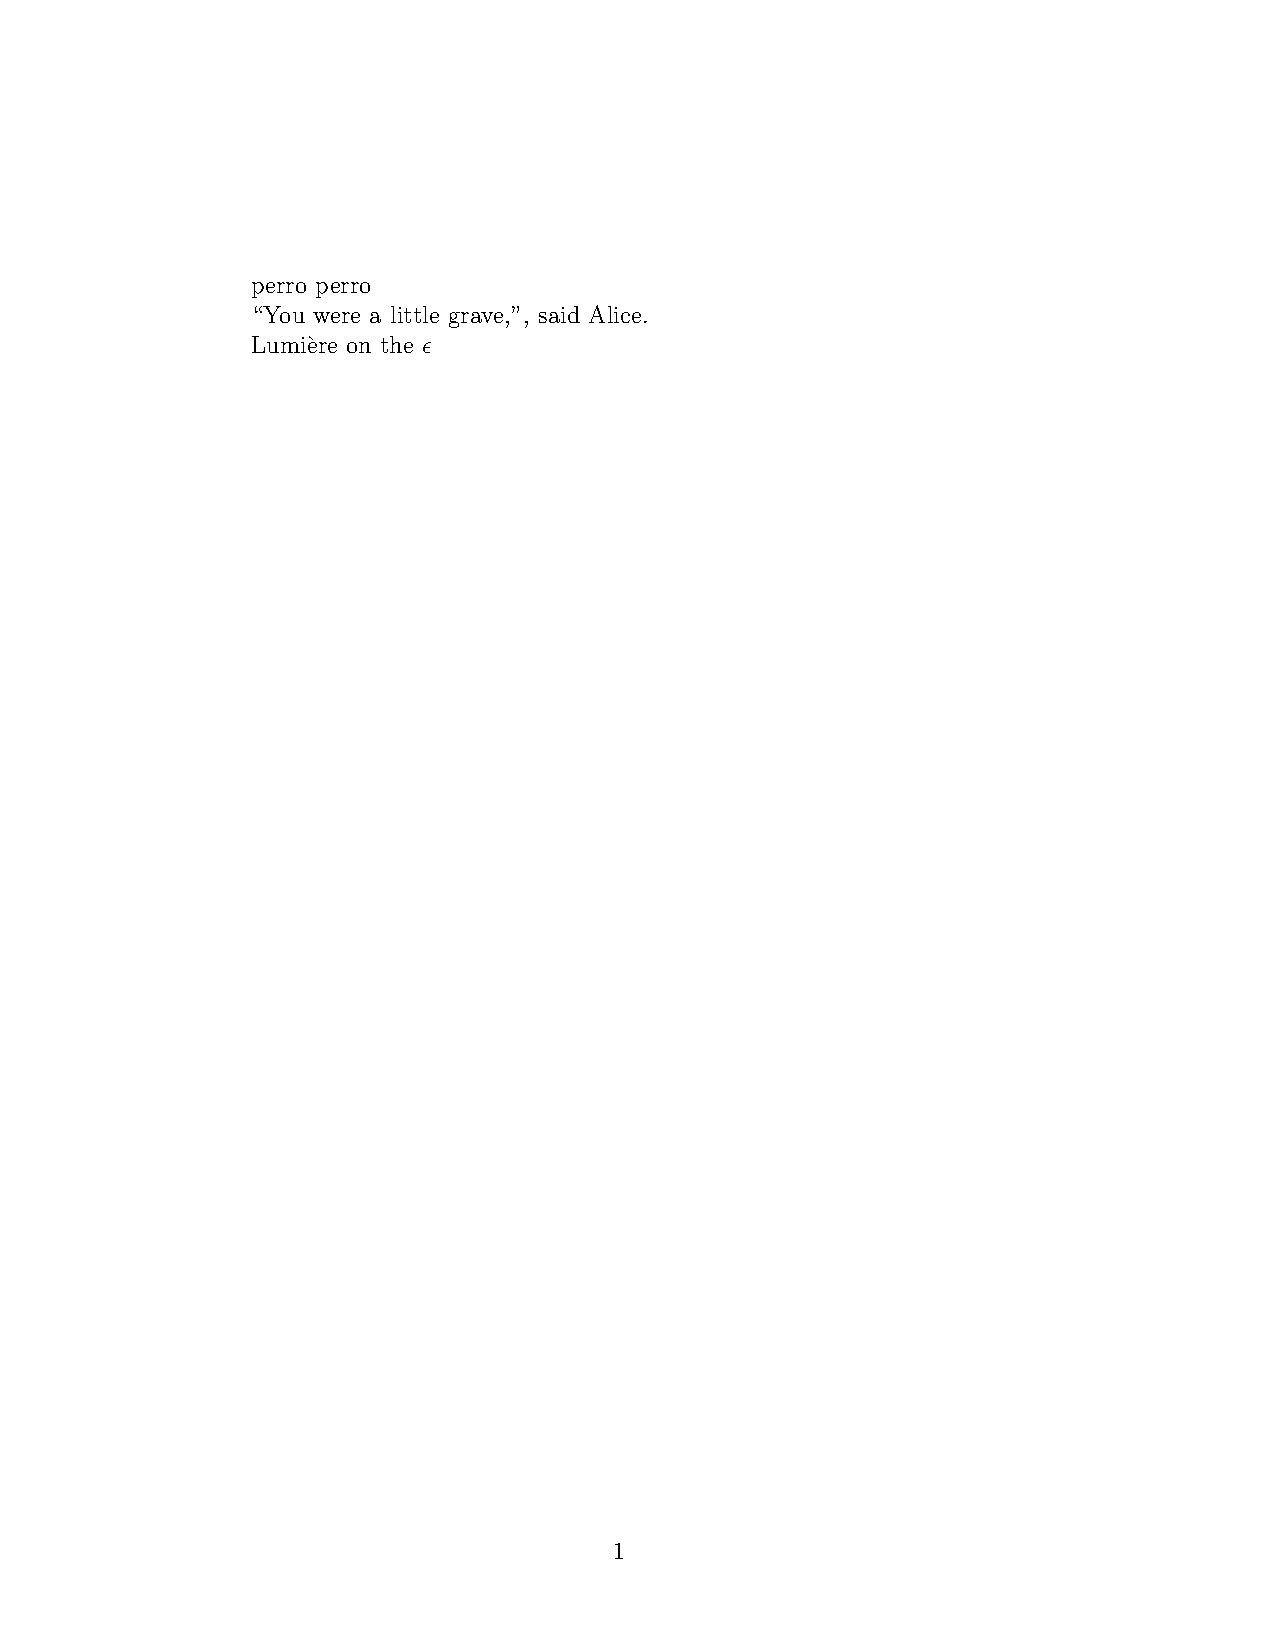
\includegraphics[width=0.8\linewidth]{test}
%\end{figure}
\end{frame}

%------------------------------------------------

\begin{frame}[fragile] % Need to use the fragile option when verbatim is used in the slide
\frametitle{Citation}
An example of the \verb|\cite| command to cite within the presentation:\\~

This statement requires citation \cite{p1}.
\end{frame}

%------------------------------------------------

\begin{frame}
\frametitle{References}
\footnotesize{
\begin{thebibliography}{99} % Beamer does not support BibTeX so references must be inserted manually as below
\bibitem[Smith, 2012]{p1} John Smith (2012)
\newblock Title of the publication
\newblock \emph{Journal Name} 12(3), 45 -- 678.
\end{thebibliography}
}
\end{frame}

%------------------------------------------------

\begin{frame}
\Huge{\centerline{The End}}
\end{frame}

%----------------------------------------------------------------------------------------

\end{document} 
